\subsection{余代数}

定义 1. A 上的余代数（或 A-余代数，若不致混淆则简称为余代数）是一个集合 E，其结构由给出以下内容来定义：

\begin{enumerate}
\def\labelenumi{(\arabic{enumi})}
\item
  E 上的一个 A-模结构；
\item
  一个 A-线性映射 \(c: \mathbf{E} \to \mathbf{E} \otimes_{\mathbf{A}} \mathbf{E}\) ，称为 \(\mathbf{E}\) 的余积。
\end{enumerate}

定义2. 给定两个余代数E、E'，其余积分别记为c和c'，从E到E'的一个态射是一个A-线性映射u：E → E'，使得

\[
(u \otimes u) \circ c = c ^ {\prime} \circ u\tag{1}
\]

换言之，它使得A-线性映射的图表可交换

\pandocbounded{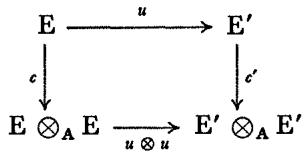
\includegraphics[keepaspectratio]{images/part004_6ed4336b.jpg}}

立即可以验证，恒等映射是态射，两个态射的复合是态射，并且每个双射态射都是同构。

示例。（1）典范同构 \(\mathbf{A} \to \mathbf{A} \otimes_{\mathbf{A}} \mathbf{A}\) (II, § 3, 第 5 号) 在 \(\mathbf{A}\) 上定义了一个 A-余代数结构。

\begin{enumerate}
\def\labelenumi{(\arabic{enumi})}
\setcounter{enumi}{1}
\item
  设 E 为一个余代数，c 为其余积，且 \(\sigma\) 为 A-模 \(E \otimes_{A} E\) 的典范自同构，使得 \(\sigma(x \otimes y) = y \otimes x\) （对 \(x \in E\) , \(y \in E\) ）；A-线性映射 \(\sigma \circ c\) 在 E 上定义了一个新的余代数结构。带此结构的 E 称为给定余代数 E 的反余代数。
\item
  设 B 为一个 A-代数，并设 \(m:B \otimes_{A} B \to B\) 为定义 B 上乘法的 A-线性映射（ \(\S 1\) ，第3号）。转置 \(^{t}m\) 于是是从 A-模 B 的对偶 \(B^{*}\) 到 \((\mathbf{B} \otimes_{\mathbf{A}} \mathbf{B})^{*}\) （即 A-模 \(B \otimes_{A} B\) 的对偶）中的一个 A-线性映射。若 B 还是有限生成的投射 A-模，则典范映射 \(\mu:B^{*} \otimes_{A} B^{*} \to (\mathbf{B} \otimes_{\mathbf{A}} \mathbf{B})^{*}\) 是一个 A-模同构（II， \(\S 4\) ，第4号）；映射 \(c = \mu^{-1} \circ ^{t}m\) 于是是一个余积，它在 A-模 B 的对偶 \(B^{*}\) 上定义了一个余代数结构。
\item
  设 X 是一个集合， \(\mathbf{A}^{(\mathbf{X})}\) 是 X 中元素以 A 中系数构成的形式线性组合的 A-模（II，§1，第11号），且 \((e_{x})_{x\in\mathbf{X}}\) 是 \(\mathbf{A}^{(\mathbf{X})}\) 的典范基。A-线性映射 \(c:A^{(\mathbf{X})}\to\mathbf{A}^{(\mathbf{X})}\otimes_{\mathbf{A}}\mathbf{A}^{(\mathbf{X})}\) 由条件 \(c(e_{x})=e_{x}\otimes e_{x}\) 定义，从而在 \(\mathbf{A}^{(\mathbf{X})}\) 上得到了一个典范余代数结构。
\item
  设 \(\mathbf{M}\) 是一个 A-模，且 \(\mathsf{T}(\mathbf{M})\) 是 \(\mathbf{M}\) 的张量代数 ( \(\S 5\) ，第1号）；根据 II， \(\S 3\) 第9号，存在且仅存在一个 A-线性映射 \(c\) ，它从 A-模 \(\mathsf{T}(\mathbf{M})\) 到 A-模 \(\mathsf{T}(\mathbf{M}) \otimes_{\mathbf{A}} \mathsf{T}(\mathbf{M})\) 中，使得对所有 \(n \geqslant 0\) ，
\end{enumerate}

\[
c (x _ {1} x _ {2} \dots x _ {n}) = \sum_ {0 \leqslant p \leqslant n} (x _ {1} x _ {2} \dots x _ {p}) \otimes (x _ {p + 1} \dots x _ {n})\tag{3}
\]

对所有 \(x_{i} \in \mathbf{M}\) ( \(x_{1}x_{2}\ldots x_{n}\) 表示代数 \(\mathsf{T}(\mathbf{M})\) 中的乘积）。这样， \(\mathsf{T}(\mathbf{M})\) 就被赋予了余代数结构。

\begin{enumerate}
\def\labelenumi{(\arabic{enumi})}
\setcounter{enumi}{5}
\tightlist
\item
  设 M 是一个 A-模，S(M) 是 M 的对称代数（§ 6，第 1 号）；从 M 到 M × M 的对角映射 \(\Delta: x \mapsto (x, x)\) 是一个 A-线性映射，因此对应着从 A-代数 S(M) 到 A-代数 S(M × M) 的一个同态 S(Δ)（§ 6，第 2 号，命题 3）。另一方面，在 § 6，第 6 号中我们定义了一个典范分次代数同构 \(h \colon \mathbb{S}(\mathbf{M} \times \mathbf{M}) \to \mathbb{S}(\mathbf{M}) \otimes_{\mathbf{A}} \mathbb{S}(\mathbf{M})\) ；通过复合，我们因此得到一个 A-代数同态
\end{enumerate}

\[
c = h \circ \mathbf {S} (\Delta): \mathbf {S} (\mathbf {M}) \rightarrow \mathbf {S} (\mathbf {M}) \otimes_ {\mathbf {A}} \mathbf {S} (\mathbf {M}),
\]

从而在 \(\mathbf{S}(\mathbf{M})\) 上定义了一个余代数结构。对所有 \(x\in \mathbf{M}\) ，根据定义 \(\mathbf{S}(\Delta)(x) = (x,x)\) ，而 § 6 第6号中给出的 \(h\) 的定义表明

\[
h ((x, x)) = x \otimes 1 + 1 \otimes x.
\]

由此可得 \(c\) 是唯一的代数同态，使得对所有 \(x \in \mathbf{M}\) ,

\[
c (x) = x \otimes 1 + 1 \otimes x.\tag{4}
\]

由于 \(c\) 是一个代数同态，因此得出：对每个序列 \((x_{i})_{1\leqslant i\leqslant n}\) （ \(n\) 个元素取自 \(\mathbf{M}\) ），

\[
\begin{array}{r l} c (x _ {1} x _ {2} \dots x _ {n}) & = \prod_ {i = 1} ^ {n} (x _ {i} \otimes 1 + 1 \otimes x _ {i}) \\ & = \sum (x _ {i _ {1}} \dots x _ {i _ {p}}) \otimes (x _ {j _ {1}} \dots x _ {j _ {n - p}}) \end{array}\tag{5}
\]

（5）式右端的求和是对所有严格递增序列（在某些情况下为空）的有序对进行的

\[
i _ {1} <   i _ {2} <   \dots <   i _ {p}, \quad j _ {1} <   j _ {2} <   \dots <   j _ {n - p}
\]

的元素组成 \([1, n]\) ，且其元素集合互补。元素 \(c(x_1 x_2 \ldots x_n)\) 是总次数为 \(n\) 的、 \(\mathbb{S}(\mathbf{M}) \otimes_{\mathbf{A}} \mathbb{S}(\mathbf{M})\) 中的元素，其双次数为 \((p, n - p)\) 的分量是

\[
\sum_ {\sigma} \left(x _ {\sigma (1)} \dots x _ {\sigma (p)}\right) \otimes \left(x _ {\sigma (p + 1)} \dots x _ {\sigma (n)}\right)\tag{6}
\]

其中求和遍历所有排列 \(\sigma\in\mathbb{S}_{n}\) ，这些排列在每个区间 \([1,p]\) 和 \([p+1,n]\) 上都是递增的。

\begin{enumerate}
\def\labelenumi{(\arabic{enumi})}
\setcounter{enumi}{6}
\tightlist
\item
  设 \(\mathbf{M}\) 是一个 A-模，对外代数 \(\bigwedge (\mathbf{M})\) 按照例 6 中对 \(\mathbb{S}(\mathbf{M})\) 的方式处理；对角映射 \(\Delta : \mathbf{M} \to \mathbf{M} \times \mathbf{M}\) 这次定义了同态 \(\bigwedge (\Delta)\) ，它从 A-代数 \(\bigwedge (\mathbf{M})\) 到 A-代数 \(\bigwedge (\mathbf{M} \times \mathbf{M})\) 中（§7，第2号，命题2）；另一方面，存在典范分次代数同构
\end{enumerate}

\[
h: \bigwedge (\mathbf {M} \times \mathbf {M}) \rightarrow \bigwedge (\mathbf {M}) ^ {\mathrm{g}} \otimes_ {\mathbf {A}} \bigwedge (\mathbf {M})
\]

（§7，第7号，命题10），因此通过复合得到代数同态 \(c = h \circ \bigwedge(\Delta): \bigwedge(M) \to \bigwedge(M)^{\mathfrak{g}} \otimes_{A} \bigwedge(M)\) ，它可视为 A-模同态 \(\bigwedge(M) \to \bigwedge(M) \otimes_{A} \bigwedge(M)\) ，从而在 \(\bigwedge(M)\) 上定义了一个余代数结构。可如同例 6 那样证明 \(c\) 是唯一的代数同态，使得对所有 \(x \in M\) ，

\[
c (x) = x \otimes 1 + 1 \otimes x,\tag{7}
\]

，因此，对每个序列 \((x_{i})_{1\leqslant i\leqslant n}\) （元素属于 \(\mathbf{M}\) ），

\[
c \left(x _ {1} \wedge x _ {2} \wedge \dots \wedge x _ {n}\right) = \left(x _ {1} \otimes 1 + 1 \otimes x _ {1}\right) \wedge \dots \wedge \left(x _ {n} \otimes 1 + 1 \otimes x _ {n}\right)
\]

其中右侧的乘积是在代数中进行的

\[
\Lambda (\mathbf {M}) ^ {\mathfrak {g}} \otimes_ {\mathbf {A}} \Lambda (\mathbf {M});
\]

为了计算这个乘积，对每对严格递增序列 \(i_1 < i_2 < \cdots < i_p\) , \(j_1 < j_2 < \cdots < j_{n-p}\) （由 \([1, n]\) 的元素组成，且其元素集合互补），考虑乘积 \(y_1y_2\ldots y_n\) ，其中 \(y_{i_h} = x_{i_h} \otimes 1 (1 \leqslant h \leqslant p)\) 和 \(y_{j_k} = 1 \otimes x_{j_k} (1 \leqslant k \leqslant n - p)\) 并且求和是对所有这些乘积进行的。由于分次代数 \(\bigwedge (\mathbf{M})^{\mathfrak{g}} \otimes_{\mathbf{A}} \bigwedge (\mathbf{M})\) 是反交换的，且元素 \(x_i \otimes 1\) 和 \(1 \otimes x_i\) 的总次数为1，根据§4，第6号，引理3和引理1，

\[
\begin{array}{r l} c (x _ {1} \wedge x _ {2} \wedge \dots \wedge x _ {n}) & = \sum (- 1) ^ {\nu} (x _ {i _ {1}} \wedge \dots \wedge x _ {i _ {p}}) \otimes (x _ {j _ {1}} \wedge \dots \wedge x _ {j _ {n - p}}) \end{array} \tag {8}
\]

其中 v 是有序对 \((h, k)\) 的个数，这些对满足 \(j_{k} < i_{h}\) ，且求和范围与 (5) 中相同。元素 \(c(x_{1} \wedge \cdots \wedge x_{n})\) 在 \(\bigwedge(\mathbf{M})^{\mathbf{g}} \otimes_{\mathbf{A}} \bigwedge(\mathbf{M})\) 中的总次数为 n，其双次数 \((p, n - p)\) 的齐次分量等于

\[
\sum_ {\sigma} \varepsilon_ {\sigma} (x _ {\sigma (1)} \wedge \dots \wedge x _ {\sigma (p)}) \otimes (x _ {\sigma (p + 1)} \wedge \dots \wedge x _ {\sigma (n)})\tag{9}
\]

求和遍历所有置换 \(\sigma\in\mathfrak{S}_{n}\) ，它们在每个区间 \([1,p]\) 和 \([p+1,n]\) 上都是递增的。

今后当我们谈到 \(\mathbf{A}^{(\mathbf{X})}\) , \(\mathsf{T}(\mathbf{M})\) , \(\mathsf{S}(\mathbf{M})\) 或 \(\bigwedge (\mathbf{M})\) 作为余代数时，除非另有说明，我们指的是分别在例 4、5、6 和 7 中定义的余代数结构。

\begin{enumerate}
\def\labelenumi{(\arabic{enumi})}
\setcounter{enumi}{7}
\tightlist
\item
  设 E, F 为两个 A-余代数，c, \(c'\) 分别为其余积。设 \(\tau:(\mathbf{E} \otimes_{\mathbf{A}} \mathbf{E}) \otimes_{\mathbf{A}} (\mathbf{F} \otimes_{\mathbf{A}} \mathbf{F}) \to (\mathbf{E} \otimes_{\mathbf{A}} \mathbf{F}) \otimes_{\mathbf{A}} (\mathbf{E} \otimes_{\mathbf{A}} \mathbf{F})\) 表示结合性同构，使得 \(\tau((x \otimes x') \otimes (y \otimes y')) = (x \otimes y) \otimes (x' \otimes y')\) 对 E 中的 \(x, x'\) 和 F 中的 \(y, y'\) 成立。则复合线性映射
\end{enumerate}

\[
\mathrm{E} \otimes_ {\mathrm{A}} \mathrm{F} \xrightarrow {c \otimes c ^ {\prime}} (\mathrm{E} \otimes_ {\mathrm{A}} \mathrm{E}) \otimes_ {\mathrm{A}} (\mathrm{F} \otimes_ {\mathrm{A}} \mathrm{F}) \xrightarrow {\tau} (\mathrm{E} \otimes_ {\mathrm{A}} \mathrm{F}) \otimes_ {\mathrm{A}} (\mathrm{E} \otimes_ {\mathrm{A}} \mathrm{F})
\]

在 A-模 E \(\otimes_{\mathbf{A}}\mathbf{F}\) 上定义了一个余代数结构，称为余代数 E 和 F 的张量积。

设 E 为一个余代数， \(\Delta\) 为一个交换幺半群。A-模 E 上的分次 \((\mathrm{E}_{\lambda})_{\lambda\in\Delta}\) 称为与 E 的余积 c 相容，如果 c 是从分次 A-模 E 到分次 A-模（ \(\Delta\) 型的 \(E\otimes_{A}E\) ）中的 0 次分次同态，换言之（II，§11，第 5 号），如果

\[
\mathrm{c} (\mathrm{E} _ {\lambda}) \subset \sum_ {\mu + \nu = \lambda} \mathrm{E} _ {\mu} \otimes_ {\mathbf {A}} \mathrm{E} _ {\nu}.\tag{10}
\]

在下文中，我们通常将注意力限制在与余积相容的 N 型分次上；带有这种分次的余代数也称为分次余代数。若 F 是另一个分次余代数，则分次余代数态射 \(\phi:E\to F\) 按定义是一个余代数态射（定义 2），同时也是分次 A-模之间的 0 次分次同态。

例。（9）显然，上述定义的余代数 \(\mathsf{T}(\mathbf{M})\) , \(\mathsf{S}(\mathbf{M})\) 和 \(\bigwedge (\mathbf{M})\) 都是分次余代数。

